\documentclass[12pt]{article}

\usepackage{amsmath}
\usepackage{graphicx}
\usepackage{verbatim}

\graphicspath{/images}

\title{Assignment 3 Workout}
\author{Thomas Vroom - i6291496}
\date{October 2022}

\begin{document}
\maketitle
\pagenumbering{gobble}

\section*{Question 1}
Let $X \sim \text{Beta}(6, 2)$.
As calculated in the previous assignment, this means the PDF of $X$ is equal to:

\[ 42x^5 - 42x^6 \]

\noindent
The CDF of $X$ can be calculated as:

\[ \int 42x^5 - 42x^6 \,dx = 7x^6 - 6x^7 \]

\noindent
Since this CDF has no gaps in it, we can calculate the median of $X$ by setting the CDF equal to $\frac{1}{2}$:

\[ 7x^6 - 6x^7 = \frac{1}{2} \]

\[ 14x^6 - 12x^7 = 1 \]

\[ 14x^6 - 12x^7 - 1 = 0 \]

\noindent
We can approximate the solution of this equation using numerical methods.
If we do this we end up with the root:

\[ x = 0.7715100364934 \]

\noindent
Thus we can conclude that Median$(X) = 0.7715100364934$.
We can confirm this is true by looking at it graphically:

\newpage
\begin{figure}[h]
    \centering
    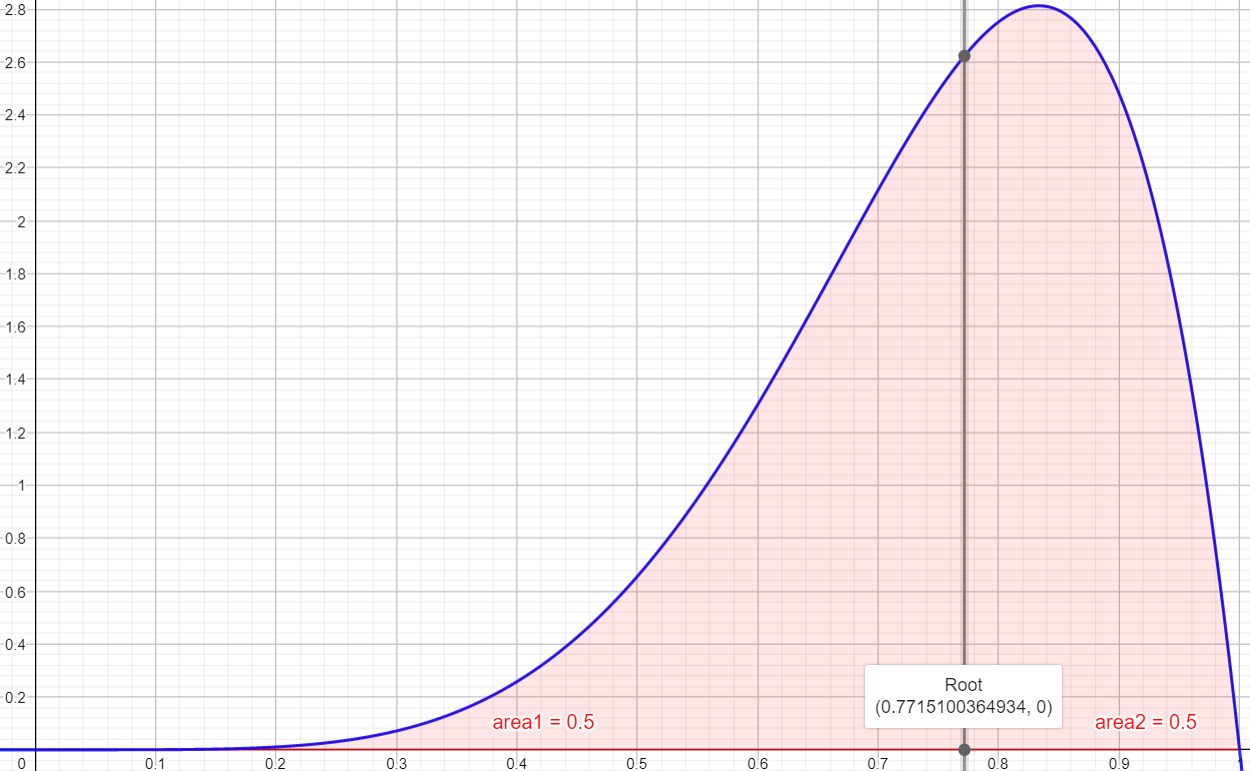
\includegraphics[scale=0.45]{images/PDF.PNG}
    \caption{The PDF of $X$. As you can see the median divides the PDF into two perfect halves with an area of $\frac{1}{2}$}
\end{figure}

\begin{figure}[h!]
    \centering
    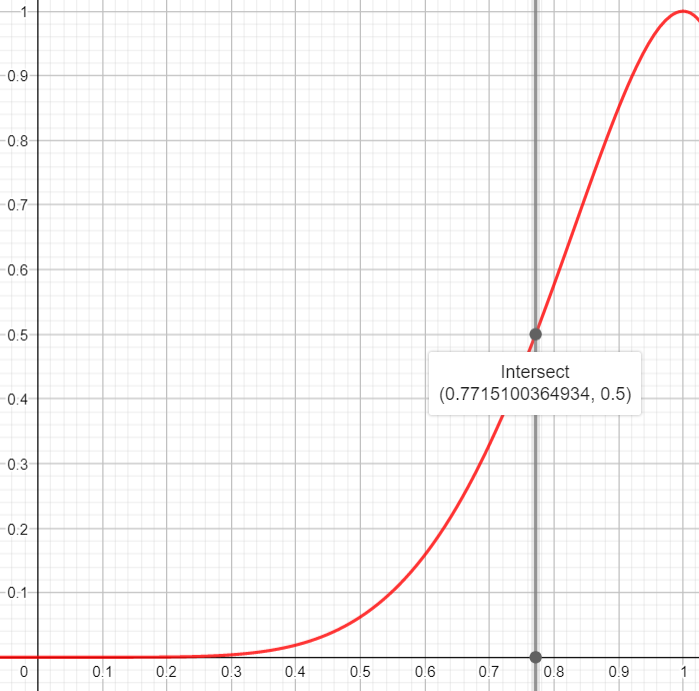
\includegraphics[scale=0.5]{images/CDF.PNG}
    \caption{The CDF of $X$. As you can see the value of the CDF equals exactly $\frac{1}{2}$ at the median}
\end{figure}

\newpage
\section*{Question 2}
The histogram produced by the bean machine is created by dropping balls down multiple layers of pins laid out in a triangle shape.
The probability of a ball going down the left or right side of a pin is $\frac{1}{2} = 0.5$, this makes this a \textbf{Bernoulli trial}.
Because each ball falls down multiple layers of pins, each with a Bernoulli trial, the total fall from top to bottom is a string of repeated Bernoulli trials.
This means that the path of each ball from top to bottom has a \textbf{binomial distribution} (repeated Bernoulli trials).
The \textbf{Central Limit Theorem} states that given a large enough sample size (in this case, number of rows), the distribution approaches a normal distribution.
This explains why the histogram created by dropping balls down many many rows of pins appears to have a normal distribution.
In formulas:

\noindent
\\
Let $X_i$ be a random variable that represents the final position of the ball.
To get to this final position, $X_i$ has to go through Bernoulli trials $Y_1, ... , Y_n$, where $n$ represents the total number of rows in the bean machine. 

\[ X_i = Y_1 + ... + Y_n \]

\[ \bar{X}_i = \frac{X_i}{n} \]

\noindent
The central limit theorem states that:

\[ \sqrt{n} \left( \frac{\bar{X}_n - \mu}{\sigma} \right) \sim \text{N}(0, 1) \]

\noindent
From this we can deduce:

\[ \sqrt{n} \left( \frac{\frac{X_i}{n} - \mu}{\sigma} \right) \sim \text{N}(0, 1) \]

\[ \frac{\frac{X_i}{n} - \mu}{\sigma} \sim \frac{1}{\sqrt{n}} \cdot \text{N}(0, 1) \]

\[ \frac{X_i}{n} - \mu \sim \frac{\sigma}{\sqrt{n}} \cdot \text{N}(0, 1) \]

\[ \frac{X_i}{n} \sim \frac{\sigma}{\sqrt{n}} \cdot \text{N}(0, 1) + \mu \]

\[ X_i \sim \frac{n \cdot \sigma}{\sqrt{n}} \cdot \text{N}(0, 1) + n \cdot \mu \]

\[ X_i \sim \sigma \sqrt{n} \cdot \text{N}(0, 1) + n \cdot \mu \]

\noindent
Which, by definition of the normal distribution, equals:

\[ X_i \sim \text{N}(n \cdot \mu, n \cdot \sigma^2) \]

\end{document}
